\documentclass[noauthor,handout]{ximera}
%handout:  for handout version with no solutions or instructor notes
%handout,instructornotes:  for instructor version with just problems and notes, no solutions
%noinstructornotes:  shows only problem and solutions

%% handout
%% space
%% newpage
%% numbers
%% nooutcomes

%I added the commands here so that I would't have to keep looking them up
%\newcommand{\RR}{\mathbb R}
%\renewcommand{\d}{\,d}
%\newcommand{\dd}[2][]{\frac{d #1}{d #2}}
%\renewcommand{\l}{\ell}
%\newcommand{\ddx}{\frac{d}{dx}}
%\everymath{\displaystyle}
%\newcommand{\dfn}{\textbf}
%\newcommand{\eval}[1]{\bigg[ #1 \bigg]}

%\begin{image}
%\includegraphics[trim= 170 420 250 180]{Figure1.pdf}
%\end{image}

%add a ``.'' below when used in a specific directory.

\newcommand{\RR}{\mathbb R}
\renewcommand{\d}{\,d}
\newcommand{\dd}[2][]{\frac{d #1}{d #2}}
\renewcommand{\l}{\ell}
\newcommand{\ddx}{\frac{d}{dx}}
\newcommand{\dfn}{\textbf}
\newcommand{\eval}[1]{\bigg[ #1 \bigg]}




\author{Jim Talamo}

\outcome{Find lengths of curves.}
\outcome{Determine whether a curve is parameterized by arclength.}
\outcome{Give a parameterization of a curve that uses arclength as a parameter.}
\outcome{Understand properties of curves that are parameterized by arclength.}
\outcome{Answer questions about arclength from a graph.}

\title[]{Arclength As A Parameter}

\newcommand{\Proj}[2]{\proj_{\vec{#2}}\vec{#1}}
\newcommand{\Scal}[2]{\scal_{\vec{#2}}\vec{#1}}
\newcommand{\Mag}[1]{\left| \vec{#1} \right|}
\newcommand{\Magf}[2]{\left| \vec{#1}\left(#2\right) \right|}
\newcommand{\Magd}[2]{\left| \vec{#1}'\left(#2\right) \right|}
\renewcommand{\vec}[1]{{\overset{\boldsymbol{\rightharpoonup}}{\mathbf{#1}}}}

\begin{document}
\begin{abstract}
\end{abstract}
\maketitle

\vspace{-0.5in}

\section{Discussion Questions}

\begin{problem}
The curve $\mathcal{C}$ traced out by  $\vec{p}(t)$ is shown below.

\begin{center}
\resizebox {4cm} {!} { 
    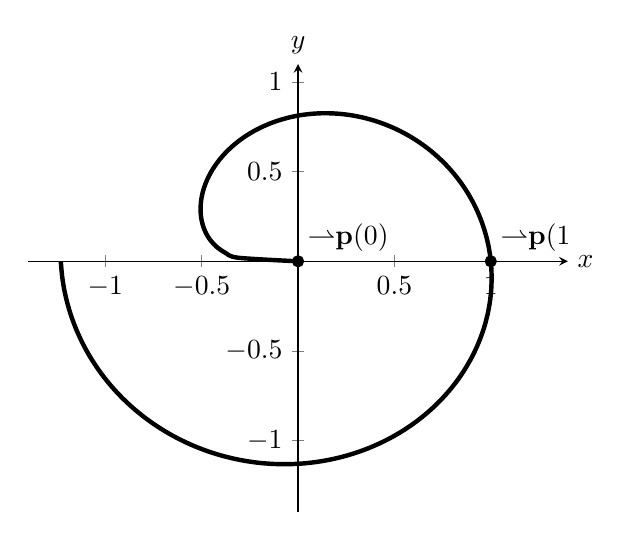
\begin{tikzpicture}
      \begin{axis}[
          xmin=-1.4, xmax=1.4, ymin =-1.4, ymax = 1.1,
          axis lines=center,  
          xlabel=$x$,  
          ylabel=$y$,  
          every axis y label/.style={at=(current axis.above origin),anchor=south},  
          every axis x label/.style={at=(current axis.right of origin),anchor=west}
        ]
        \addplot [black,ultra thick,domain=0:360,smooth,samples=100] ({-((x/180)^(.3))*cos(x)},{((x/180)^.3)*sin(x)});
        \node[above right,black] at (axis cs: 0,0) {$\vec{p}(0)$};
        \node[above right,black] at (axis cs: {-((180/180)^(.3))*cos(180)},{((180/180)^.3)*sin(180)}) {$\vec{p}(1)$};
        

        \addplot[color=black,fill=black,only marks,mark=*] coordinates{(-{((180/180)^(.3))*cos(180)},{((180/180)^.3)*sin(180)})};
        \addplot[color=black,fill=black,only marks,mark=*] coordinates{(0,0)};
        
      \end{axis}
    \end{tikzpicture}}
\end{center}

I. Give a vector parallel to $\vec{p}(1)$ whose magnitude is $3$.

II. Sketch a tangent vector to the curve at the point associated to $\vec{p}(1)$.

III. Explain whether the $\vec{p}(t)$ is a parameterization of the curve that uses arc length as a parameter.


\begin{freeResponse}  
We use the graph of the given curve to answer these questions.

\textbf{I.} Note that $\vec{p}(1) = \vector{1,0}$, so a vector parallel to $\vec{p}(1)$ of magnitude $3$ is $\vector{3,0}$.  Note that $\vector{-3,0}$ is also such a vector.

\textbf{II.} A tangent vector to the curve should be parallel to the curve at the point associated to $\vec{p}(1)$.  

\begin{center}
\resizebox {4cm} {!} { 
    \begin{tikzpicture}
      \begin{axis}[
          xmin=-1.4, xmax=1.4, ymin =-1.4, ymax = 1.1,
          axis lines=center,  
          xlabel=$x$,  
          ylabel=$y$,  
          every axis y label/.style={at=(current axis.above origin),anchor=south},  
          every axis x label/.style={at=(current axis.right of origin),anchor=west}
        ]
        \addplot [black,ultra thick,domain=0:360,smooth,samples=100] ({-((x/180)^(.3))*cos(x)},{((x/180)^.3)*sin(x)});
        \node[above right,black] at (axis cs: 0,0) {$\vec{p}(0)$};
        \node[above right,black] at (axis cs: {-((180/180)^(.3))*cos(180)},{((180/180)^.3)*sin(180)}) {$\vec{p}(1)$};

        \addplot[penColor,->,ultra thick] coordinates{(-{((180/180)^(.3))*cos(180)+.01},{((180/180)^.3)*sin(180)}) (-{((180/180)^(.3))*cos(180)+.01},{((180/180)^.3)*sin(180)-.8})};        

        \addplot[color=black,fill=black,only marks,mark=*] coordinates{(-{((180/180)^(.3))*cos(180)},{((180/180)^.3)*sin(180)})};
        \addplot[color=black,fill=black,only marks,mark=*] coordinates{(0,0)};
        
      \end{axis}
    \end{tikzpicture}}
\end{center}

\textbf{III.} If a curve uses arc length as a parameter, then for any $s$ in the domain of the curve, $\vec{p}(s)$ is the position of a point on the curve after traveling $s$ units from the starting point.  

Since $\vec{p}(0)=\vector{0,0}$, if the curve were parameterized by arc length, $\vec{p}(1)$ would give the point on the curve after traveling $1$ unit along the curve.  However, the only way to travel $1$ unit from $(0,0)$ to $(1,0)$ is to travel along the $x$-axis.  From the picture, we thus have that the length of the segment of the curve from $(0,0)$ to $(1,0)$ is longer than $1$ unit.  Thus, the curve does not use arc length as a parameter.  

\end{freeResponse}


\end{problem}


%%%%%%%%%%%%%%%%%%%%%%%%%%%%%%%%%%%%%%%%%%%%%%%%%%%

\begin{problem}
Consider the graph below of the vector-valued
function $\vec{p}(s)$ and suppose that $\vec{p}(s)$ is
an arclength parameterization.   %Thanks to bart Snapp for this

\begin{center}
\resizebox {6cm} {!} { 
    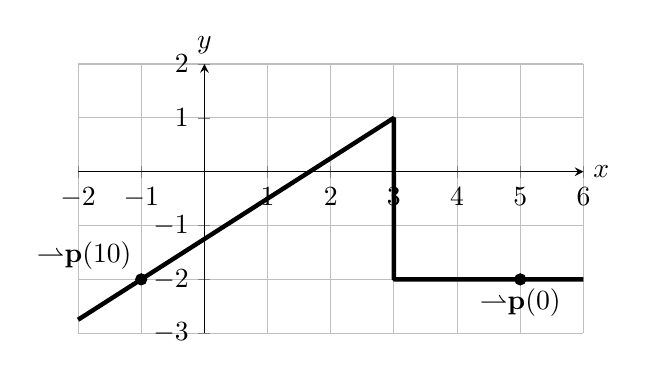
\begin{tikzpicture}
      \begin{axis}%
        [
	  xmin=-2,xmax=6,
          ymin=-3,ymax=2,
          xlabel=$x$,ylabel=$y$,
          axis lines=center,
          every axis y label/.style={at=(current axis.above origin),anchor=south},
          every axis x label/.style={at=(current axis.right of origin),anchor=west},
          clip=false,
	  grid =major,
          width=8cm,
          height=5cm,
          xtick={-2,-1,...,6},
          ytick={-3,-2,...,2},
	]
        \addplot[line join =bevel,black,ultra thick] coordinates{
          (-2,-2.75) (3,1) (3,-2) (6,-2)
        };
        \addplot[color=black,fill=black,only marks,mark=*] coordinates{(5,-2)};  %% closed hole
        \addplot[color=black,fill=black,only marks,mark=*] coordinates{(-1,-2)};  %% closed hole
        \node[black,below] at (axis cs: 5,-2) {$\vec{p}(0)$};
        \node[black,above left] at (axis cs: -1,-2) {$\vec{p}(10)$};
      \end{axis}
    \end{tikzpicture}}
\end{center}

I. Compute $\vec{p}(5)$.

II. Compute $\int_0^{10} \vec{p}'(s)\dotp\vec{p}'(s)\d s$.

\begin{freeResponse}
Note that if a curve traced out by $\vec{p}(t)$ uses arc length as a parameter, and we take $s(0)=0$, we know two important facts.

\begin{itemize}
\item[1.] $\int_0^s \left|\vec{r}'(t)\right| \d t = s$; that is, the length of the segment of the curve from $t=0$ to $t=2$ is exactly $s$.
\item[2.] $ \left|\vec{r}'(t)\right| = 1 $ for all $t$; that is, the curve is traced out with unit speed.
\end{itemize} 

\textbf{I.} To find $\vec{p}(5)$, we must travel $5$ units along the curve form $\vec{p}(0)$.  After traveling for $5$ units, we arrive at $(3,1)$, so $\vec{p}(5) = \vector{3,1}$.

\textbf{II.} Note that for any vector $\vec{v}$, $\Mag{v}^2 = \vec{v} \dotp \vec{v}$, so $\vec{p}'(s)\dotp\vec{p}'(s) = \left|\vec{p}'(s)\right|^2$.  Since the curve is parameterized by arc length, we have that $\left|\vec{p}'(s)\right| =1$, so 

\[
\int_0^{10} \vec{p}'(s)\dotp\vec{p}'(s)\d s = \int_0^{10} \left|\vec{p}'(s)\right|^2 \d s= \int_0^{10} 1 \d s = \eval{s}_0^{10} = 10. 
\]
\end{freeResponse}
\end{problem}


%%%%%%%%%%%%%%%%%%%%%%%%%%%%%%%%%%%%%%%%%%%%%%%%%%%

%
%\begin{problem}
%Two students watch a particle move counterclockwise in a circle of radius $4 \unit{ft}$, centered at the origin, at a rate of $.1 \unit{rad/sec}$, and the ball originally starts at $(x,y)=(4,0)$, where $x$ and $y$ are measured in \unit{ft}.  Student 1 decides to describe the location of the ball in $\unit{ft}$ and gives a parameterization
%\[
%\vec{r}(t) = \vector{4\cos(\omegat)
%\]   
%\begin{freeResponse}
%
%\end{freeResponse} 
%\end{problem}

%%%%%%%%%%%%%%%%%%%%%%%%%%%%%%%%%%%%%%%%%%%%%%%%%%%

\section{Group Work}

\begin{problem}
Determine if the following statements are true or false and explain your response.

I. If $\vec{F}$ is a nonzero vector and $\vec{p}(s), s \geq 0$ gives an arc length parameterization of a curve, then for \emph{any} $s\geq 0$, $\scal_{\vec{p}(s)}\vec{F} = \vec{F} \dotp \vec{p}(s)$.

II. The curve $\mathcal{C}$ is traced out by the $\vec{r}(t)=\vector{\frac{2}{3}t^{3/2}, \frac{1}{2}t}, t \geq0$.  

Since $\vec{r}'(t) = \vector{t^{1/2},\frac{1}{2}}$, we have that $\left|\vec{r}'(t)\right| = \sqrt{t+\frac{1}{4}}$. 

Hence, the curve is parameterized by arc length since $\left|\vec{r}'(t)\right|=1$ when $t=\frac{3}{4}$.

III. Suppose a curve is traced out by a differentiable vector-valued function $\vec{p}(t)$ and it is known that this is an arc length parameterization.  Then, the \emph{unit} tangent vector to the curve is given by $\uvec{T}(t) = \vec{r}'(t)$. 

\begin{freeResponse}
Recall a few important facts about arc length; if a curve traced out by $\vec{p}(t)$ uses arc length as a parameter, and $s(0)=0$, we know two important facts.

\begin{itemize}
\item[1.] $\int_0^s \left|\vec{r}'(t)\right| \d t = s$; that is, the length of the segment of the curve from $t=0$ to $t=2$ is exactly $s$.
\item[2.] $ \left|\vec{r}'(t)\right| = 1 $ for all $t$; that is, the curve is traced out with unit speed.
\end{itemize} 


\textbf{I.} This statement is false.

\[ \scal_{\vec{p}(s)}\vec{F} = \frac{ \vec{F} \dotp \vec{p}(s)}{\Magf{p}{s}} \]

While $\left|\vec{p}'(s)\right| = 1$,  $\Magf{p}{s}$ is the distance from the origin to the point associated to $\vec{p}(s)$, which so $\Magf{p}{s} \neq 1$ for all $s$.

\textbf{II.} This statement is false.  

It is true that if $\vec{r}(t)=\vector{\frac{2}{3}t^{3/2}, \frac{1}{2}t}$, then $\vec{r}'(t) = \vector{t^{1/2},\frac{1}{2}}$ and $\left|\vec{r}'(t)\right| = \sqrt{t+\frac{1}{4}}$.  In order for the curve to be parameterized by arc length, we need that $\Magf{r}{t} = 1 $ for \emph{all} $t$, not just for one particular one.

\textbf{III.} This is true.  

In general, the unit tangent vector is given by

\[
\uvec{T}(t) = \frac{\vec{r}'(t)}{\left|\vec{r}'(t)\right|}.
\]
Since the curve is parameterized by arc length, we have that $\left|\vec{r}'(t)\right| = 1$ for all $t$, so 

\[
\uvec{T}(t) = \frac{\vec{r}'(t)}{\left|\vec{r}'(t)\right|}=\frac{\vec{r}'(t)}{1} = \vec{r}'(t).
\] 

 \end{freeResponse}
\end{problem}

%%%%%%%%%%%%%%%%%%%%%%%%%%%%%%%%%%%%%%%%%%%%%%%%%%%


\begin{problem}
The curve $\mathcal{C}$ is traced out by the vector-valued function \[ \vec{r}(t) = \vector{1-2t, 2t^{3/2},6t^{3/2}}, 0 \leq t \leq 2.\]   

I. Determine whether the curve is parameterized by arc length.  If it is not, give a parameterization $\vec{p}(s)$ that uses arc length as a parameter.  Don't forget to include the domain of the arc length parameter $s$.

II. Find $\left|\vec{p}'(s)\right|$ when $s=\sqrt{2}$.

III. What is the length of $\mathcal{C}$?

\begin{freeResponse}
In order to check whether the curve uses arc length as a parameter, we compute $\left|\vec{r}'(t)\right|$.  Note

\[
\vec{r}'(t) = \vector{-2, 3 t^{1/2}, 9t^{1/2}},
\]

so 

\[
\Magd{r}{t} = \sqrt{4+9t+81t} = \sqrt{4+90t}.
\]

Since $\Magd{r}{t} \neq 1$ for all $t$, the curve does not use arc length as a parameter.  To give a description that does, we do the following.

\begin{itemize}
\item[1.] Find $s$ in terms of $t$ by computing $s = \int_0^t \left|\vec{r}'(\tau)\right| \d \tau$.

Since $\left|\vec{r}'(t)\right| = \sqrt{4+90t}$, $\left|\vec{r}'(\tau)\right| = \sqrt{4+90\tau}$, and thus

\begin{align*}
s &= \int_0^t \left|\vec{r}'(\tau)\right| \d \tau \\
&= \int_0^t \sqrt{4+90\tau} \d \tau
\end{align*}

Note that we need to find the antiderivative $\int \sqrt{4+90x} \d x$ to proceed, and by performing the substitution $u=4+90x$ if necessary,

\[
\int \sqrt{4x+90} \d x = \frac{1}{135} (4+90x)^{3/2} +C.
\] 

Thus, we find that $s(t) = \eval{\frac{1}{135} (4+90\tau)^{3/2}}_0^t = \frac{1}{135} (4+90t)^{3/2}-\frac{8}{135}$.


\item[2.] Solve for $t$ in terms of $s$.

This requires some careful algebra so let's work through it one step at a time.

\begin{align*}
s &= \frac{1}{135} (4+90t)^{3/2}-\frac{8}{135} \\
s +\frac{8}{135} &=  \frac{1}{135} (4+90t)^{3/2} \\
135s +8 &= (4+90t)^{3/2}  \\
\left(135s+8 \right)^{2/3} &= 4+90t \\
t &= \frac{\left(135s+8 \right)^{2/3} -4}{90} .
\end{align*}



\item[3.] We can now find the parameterization $\vec{p}(s)$ by substituting the expression above for $t$ in the original parameterization. 

\begin{align*}
\vec{r}(t) &= \vector{1-2t, 2t^{3/2},6t^{3/2}}, 0 \leq t \leq 2. \\
\vec{p}(s) &= \vector{1-2\left[ \frac{\left(135s+8 \right)^{2/3} -4}{90} \right], 2\left[ \frac{\left(135s+8 \right)^{2/3} -4}{90} \right]^{3/2},6\left[ \frac{\left(135s+8 \right)^{2/3} -4}{90} \right]^{3/2}}\\
\end{align*} 

Note that we also need to transform the domain as well.  Since the original domain is $0 \leq t \leq 2$, we have $0 \leq  \frac{\left(135s+8 \right)^{2/3} -4}{90} \leq 2$, or 

\[
\textrm{ Domain in } s: ~ 0 \leq s \leq\frac{1}{135}\left[(184)^{3/2}-8\right]
\]
\end{itemize}

\textbf{II.} Since $\vec{p}(s)$ is a parameterization that uses arc length as a parameter, we have that $\Magd{p}{s} =1$ for all $s$, so $\Magd{p}{s} =1$ when $s = \sqrt{2}$.

\textbf{III.} The length of $\mathcal{C}$ can be found from the domain of the arc length parameter; since the curve is defined for $0 \leq t \leq 2$ and $s(2) = \frac{1}{135}\left[(184)^{3/2}-8\right]$, the length of the curve is $\frac{1}{135}\left[(184)^{3/2}-8\right] \unit{units}$.

\end{freeResponse}
\end{problem}


%%%%%%%%%%%%%%%%%%%%%%%%%%%%%%%%%%%%%%%%%%%%%%%%%%%

\begin{problem}
The curve $\mathcal{C}$ traced out by the vector-valued function \[ \vec{r}(t) = \vector{3\cos(\omega t^2), -3\sin(\omega t^2)}, 0 \leq t \leq 2\pi. \]

Find a value of $\omega$ so the curve is parameterized by arc length or explain why no such value for $\omega$ exists.

\begin{freeResponse}
Since $\vec{r}(t) = \vector{3\cos(\omega t^2), -3\sin(\omega t^2)}$, $\vec{r}'(t) = \vector{-6t \sin(\omega t^2), -6t\cos(\omega t^2)}$, and thus

\[
\Magd{r}{t} = \sqrt{36t^2\sin^2(\omega t^2) + 36t^2 \cos^2(\omega t^2)} = \sqrt{36t^2\left[\sin^2(\omega t^2) + \cos^2(\omega t^2)\right]} = 6t.
\]

Since $\Magd{r}{t} \neq 1$ for all $t$, the curve does not use arc length as a parameter for any value of $\omega$.

\begin{remark}
Try animating the curve on Desmos; you should see that the parameterization traces out a circle and the sped increases as a function of $t$.  There is no value of $\omega$ that will make the curve have uniform speed, so the curve is not parameterized by arc length for any choice of $\omega$.
\end{remark}
\end{freeResponse}
\end{problem}

%%%%%%%%%%%%%%%%%%%%%%%%%%%%%%%%%%%%%%%%%%%%%%%%%%%

\begin{problem}
Suppose that $a>0$ and the curve $\mathcal{C}$ traced out by the vector-valued function \[ \vec{r}(t) = \vector{\frac{1}{3}t^3, 1+2t^2}, 0 \leq t \leq a. \]

I. Find a value of $a$ so the curve uses arc length as a parameter or explain why no such $a$-value exists.

II. Find a value of $a$ so the length of the curve is $5$ or explain why no such $a$-value exists.

\begin{freeResponse} 
\textbf{I.} Note that $\vec{r}'(t)$ is independent of $a$, the choice of $a$ will not affect whether the curve is parameterized by arc length.  Noting that  $\vec{r}'(t) = \vector{3t^2, 4t}$, have that $\Magd{r}{t} = \sqrt{9t^4+16t^2}$, so the curve is not parameterized by arc length since $\Magd{r}{t} \neq 1 $ for all $t$.

\textbf{II.}
The length of the curve is given by 

\begin{align*}
s = \int_0^a \Magd{r}{t} \d t  &= \int_0^a \sqrt{9t^4+16t^2} \d t \\
&= \int_0^a \sqrt{t^2 \cdot \left(9t^2+16\right)} \d t \\
&=  \int_0^a \sqrt{t^2} \cdot \sqrt{9t^2+16} \d t \\
&=  \int_0^a t \cdot \sqrt{9t^2+16} \d t \qquad \textrm{ (since } t \geq 0 \textrm{ for } 0 \leq t \leq 2, \sqrt{t^2} = t)\\
&=\eval{\frac{1}{27}(9t^2+16)^{3/2} }_0^a \\
&=\frac{1}{27}(9a^2+16)^{3/2}-\frac{64}{27}
\end{align*}

To find the desired value for $a$, set $s=5$ and solve for $a$.

\begin{align*}
\frac{1}{27}(9a^2+16)^{3/2}-\frac{64}{27}&=5 \\
(9a^2+16)^{3/2}-64&=135 \\
(9a^2+16)^{3/2}&=199 \\
9a^2+16&=(199)^{2/3} \\
a^2&=\frac{(199)^{2/3}-16}{9} \\
a&=\pm\sqrt{\frac{(199)^{2/3}-16}{9}} \\
\end{align*}

Since we need $a>0$, choose $a=\frac{\sqrt{(199)^{2/3}-16}}{3}$.
\end{freeResponse}
\end{problem}

%%%%%%%%%%%%%%%%%%%%%%%%%%%%%%%%%%%%%%%%%%%%%%%%%%%


\end{document}
